\section{Collocation Analysis}
\label{sec:collocation}


\begin{figure*}
  \centering
\begin{subfigure}{\linewidth}
  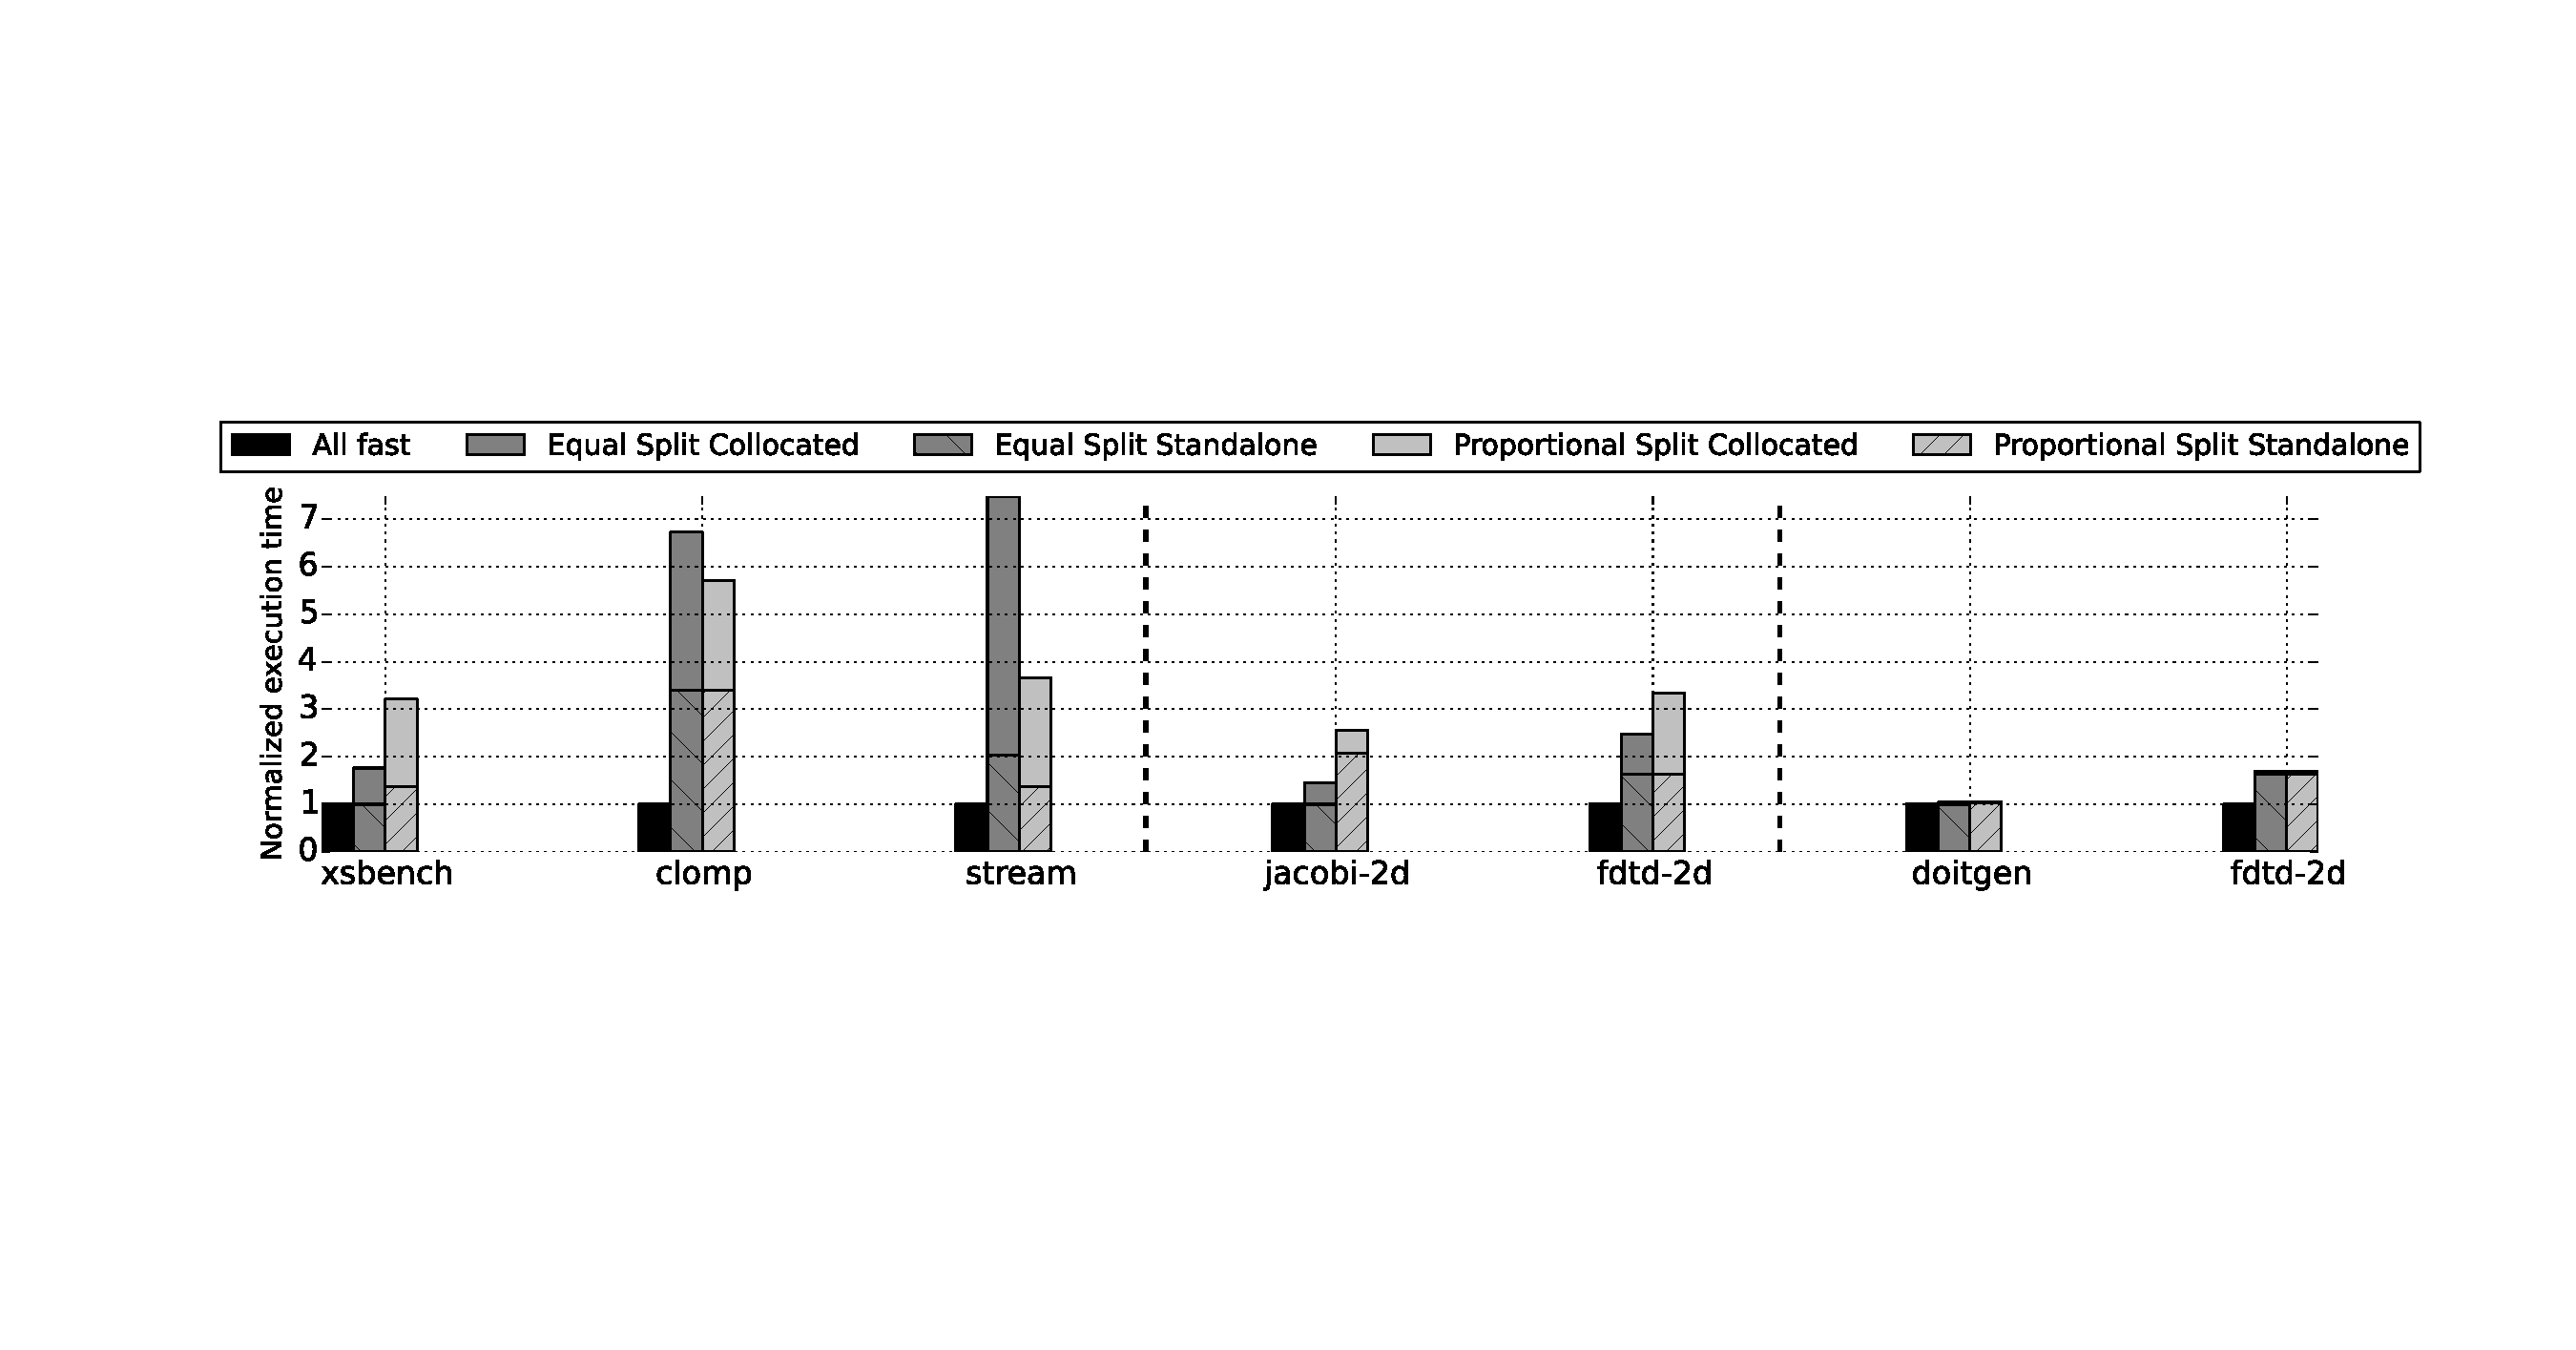
\includegraphics[width=\linewidth]{figures/tiering1.pdf}
      \captionsetup{labelformat=empty}
\caption{Execution time slowdown from `all-in-DRAM' for three different collocation combinations (separated with dashed lines). The shaded parts refer to the slowdown caused by data tiering. The unshaded parts depict the additional slowdown due to collocation. }
%  \label{fig:static}  
  \end{subfigure}

   \begin{subfigure}{\linewidth}
  \begin{subfigure}{0.425\linewidth}
  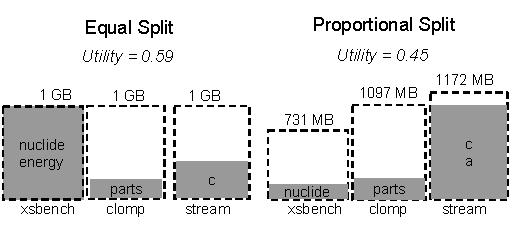
\includegraphics[width=\linewidth]{figures/tiering1a.pdf}
      \captionsetup{labelformat=empty}
  \caption{Collocation of XSBench, CLOMP, STREAM}
    \end{subfigure}%  
     \begin{subfigure}{0.3\linewidth}
  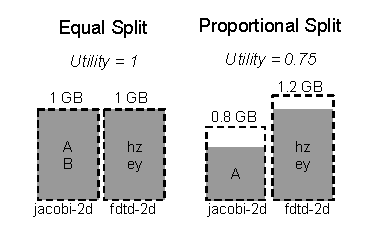
\includegraphics[width=\linewidth]{figures/tiering1b.pdf}
      \captionsetup{labelformat=empty}
    \caption{Collocation of jacobi-2d, fdtd-2d}
    \end{subfigure}%  
     \begin{subfigure}{0.3\linewidth}
     \centering
  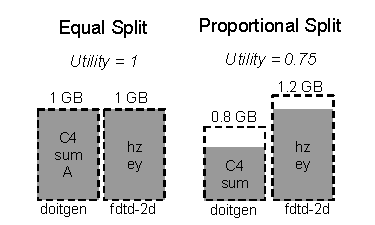
\includegraphics[width=\linewidth]{figures/tiering1c.pdf}
      \captionsetup{labelformat=empty}
    \caption{Collocation of doitgen, fdtd-2d}
    \end{subfigure}  
          \captionsetup{labelformat=empty}
  \caption{Utility and objects allocated in FastMem. The total available FastMem capacity is the sum of the private partitions of each application.}
  \end{subfigure}
  \caption{Comparison of equal and proportional capacity split schemas for three different collocation combinations.}
  \label{fig:tiering1}
    \vspace{-0.1in}
\end{figure*}

Data tiering techniques are able to mitigate the performance slowdown of an application, that spans its dataset across heterogeneous memory components, 
by occupying all the available FastMem and servicing with lower latency as many memory requests as possible. However, in the case of multi-tenant environments, the available FastMem will be yet another resource that needs to be fairly and optimally distributed across co-running applications.

In this section, we first experiment with techniques that divide the total available FastMem across the co-running kernels and evaluate their effectiveness. Then, based on the observations made in Section~\ref{sec:analysis}, regarding the sensitivity to slow memory on an application as well as data structure level, we further refine the tiering solutions for collocated workloads, proposing memory-sharing techniques. 

The performance of the proposed techniques across the CORAL and Polybench benchmarks is depicted in Figures~\ref{fig:tiering1},~\ref{fig:tiering2} and their effectiveness is  summarized in Table~\ref{tbl:tiering_summary} for the CORAL benchmarks.
We evaluate the effectiveness of all schemas, using the following criteria: 
\begin{tightenumerate}
\item The total runtime slowdown of an application when running in collocation, compared to standalone execution with all data allocated in FastMem (`All fast'). One part of this slowdown is attributed to SlowMem accesses due to data tiering and the other part captures the absolute impact of execution over shared resources. A technique that is able to highly mitigate this slowdown across most collocated applications is more efficient compared to the others.
\item The aggregate utilization of FastMem from all collocated applications. We define \(FastMem\ Utility = \frac{Bytes\ Allocated}{Capacity}\). Utility can be less than 1, if the workload size exceeds the FastMem capacity, due to the assumption that there is no support for partial object allocations, thus if a data structure doesn't fit into the available FastMem, it cannot be placed there, giving its position to the next object 
in the order determined by the benefit factors. High FastMem utility shows that the schema is able to make efficient use of the available FastMem and that will translate to higher application performance.\\
\end{tightenumerate}

\noindent All following techniques are static, because they assume that applications will first need to execute the offline profiling phase, that will determine the priority order for FastMem allocations of the different data objects, and then start execution using the part of FastMem they're entitled to. The partitioning schemas also require prior knowledge of the number of collocated applications, so as to define the amount of partitions. 

%%%%%%%%%%%%%%%%%%%%%%% Static Partitioning %%%%%%%%%%%%%%%%%%%%%%%%%%%%%%%%
\subsection{Static Partitioning}
\label{subsec:static}
Existing data tiering solutions, described in Section ~\ref{sec:intro},
can be directly applied into a shared heterogeneous memory system, when partitioning the available FastMem into parts private to each application. We experiment with the following predominant schemas to partition a shared resource.\\
\noindent{\bf Equal Capacity Split.}
This technique divides the available FastMem into parts that are equal for every application. More specifically, the available FastMem of total capacity C will be split into 
N parts of size $\frac{C}{N}$ for each out of the N workloads. It ensures fair partitioning of the available FastMem across the collocated applications. 

\noindent{\bf Propotional Capacity Split.}
This schema splits the available FastMem into parts that are proportional to the overall workload sizes. In more detail, if FastMem has total capacity C and 
each out of the N applications has size $S_i$, then FastMem will be divided into parts of size $C*\frac{S_i}{\sum_{i=1}^{N}S_i}$. This provides fairness on an application level and 
accounts for maximizing the FastMem utility, by adjusting the FastMem partitions to the application memory demands. \\

%\begin{table}[ht]
%\centering
%  \begin{tabular}{|p{1.2cm}||p{3cm}||p{3cm}|} \hline
%    Kernel & Equal split & Proportional Split \\\hline \hline
%    jacobi-2d 	& A (F) > B (F) &  A (F) > B (S) \\\hline
 %   fdtd-2d 	& hz (F) > ey (F) > ex (S) & hz (F) > ey (F) > ex (S) \\\hline
 %   doitgen 	& C4 (F) > sum (F) > A (F) & C4 (F) > sum (F) > A (S) \\\hline
 %   xsbench 	& nuclide (F) > energy (F) & nuclide (F) > energy (S) \\\hline
 %   clomp	 	& zones (S) > parts (F) & zones (S) > parts (F) \\\hline
%    stream 		& c (F) > a (S) > b (S) & c (F) > a (F) > b (S) \\\hline
 % \end{tabular}
%  \caption{Data tiering due to the capacity restrictions of the equal and proportional capacity split schemas. (F) indicates object allocation in FastMem, (S) in SlowMem.}
 % \label{tbl:tiering_split}
 % \vspace{-0.3in}
%\end{table}


%\subsubsection
\vspace{0.6ex}
\noindent{\bf\em CORAL Experiments}
\vspace{0.3ex} 

\noindent First, we experiment with three of the skeleton benchmarks in the CORAL suite. We collocate all three 
applications of 4.1 GB aggregate memory footprint, over 3 GB of shared FastMem and 4 GB of SlowMem.
The individual working set sizes are 1 GB for XSBench, 1.5 GB for CLOMP and 1.6 GB for STREAM, as shown in Table 
~\ref{tbl:tiering}. The partition sizes are 1 GB for each benchmark in the case of the equal capacity split method. 
For the proportional capacity split schema XSBench gets 731 MB of FastMem, CLOMP 1097 MB and STREAM 1172 MB. The objects allocated in FastMem for every collocated application are depicted in Figure ~\ref{fig:tiering1}. 
In addition, we run these three multi-threaded applications using 4 instead of 12 threads, so that when all three are 
co-executing they do not exceed the available cores on the node. In this way, we can eliminate other 
slowdown factors due to thread CPU scheduling and capture the overhead of sharing the hardware caches and 
memory subsystem. Furthermore, in order to account for the different run times of the three applications and 
the non-sensitive initialization phase of XSBench, we report the average run time of each one, excluding the very first and last run. Figure ~\ref{fig:tiering1} shows the slowdown of the applications due to data tiering and collocation.

First, we observe that XSBench runs faster in the equal capacity split schema, due to the fact that all of its dataset fits in FastMem. Additionally, in the case of the proportional capacity split, most of its slowdown comes from the collocation rather than the data tiering itself, due to the fact that the object that is now allocated in SlowMem, has trivial benefit factor. However, the allocation of the low benefit factor object of significant size (970 MB) in SlowMem, incurs up to 1.5x additional slowdown.

Second, although CLOMP has the same data tiering in both partitioning schemas, it gets to run faster in the case of proportional capacity split. This can most likely be	 attributed to the fact that there is extra bandwidth available to use from the SlowMem, due to the data tiering imposing more data allocations, thus accesses to FastMem, than in the equal capacity scplit.

Third, STREAM incurs bigger slowdown in the case of equal capacity split, due to the capacity restriction allowing to allocate only one object in FastMem. Also, most of its slowdown comes from collocation rather than data tiering, further highlighting the impact of SlowMem accesses in shared execution environments.

Finally, the equal capacity split schema accounts for 0.59 of FastMem utility, compared to 0.45 in the proportional capacity split. In both cases, the utility is very restricted and shows the limitation of partitioning techniques to make clever data placement decisions, something that is reflected in the significant application slowdown imposed by collocation for the given data tierings.
 
 \begin{table*}[t]
\centering
  \begin{tabular}{|p{1.5cm}|p{2cm}|p{9cm}|p{2.2cm}|p{1.2cm}|} \hline
	Category & Name & Technique & Slowdown from `all-in-FastMem' & FastMem utility    \\\hline \hline
    \multirow{2}{*}{Partitioning} & Equal Capacity Split & Creates equal partitions of FastMem across collocated kernels. Each kernel places objects to their partition, in descending benefit factor order.  & up to 7x & 0.59 \\\cline{2-5}
    & Proportional Capacity Split & Partitions FastMem in parts proportional to the individual workload sizes. Each kernel places objects to their partition, in descending benefit factor order. & up to 6x & 0.45\\\hline
        \multirow{3}{*}{Sharing} & Fair Merge & Places objects in FastMem following the descending benefit factor order, choosing from a different application at a time.  & up to 2.7x & 0.87\\\cline{2-5}
    & Blind Merge & Places objects in FastMem following the descending benefit factor absolute order of all applications. & up to 2.6x & 0.96 \\\cline{2-5}
    & {\bf CoMerge} & Places objects in FastMem following the descending {\it co-benefit factor} absolute order of all applications. Has the same effect with Blind Merge for kernels in the same sensitivity level. & up to 2.6x & 0.96 \\\hline
  \end{tabular}
  \caption{Summary and comparison of the effectiveness of data tiering techniques across the collocated CORAL benchmarks. Since these kernels belong to the same sensitivity level, Blind Merge and CoMerge have the same effect. Memory sharing techniques are efficient because they can significantly mitigate the runtime slowdown due to the higher FastMem utility.}
  \label{tbl:tiering_summary}
    \vspace{-0.3in}
\end{table*}


%\subsubsection
\vspace{2ex}
\noindent{\bf\em Polybench Experiments}
\vspace{0.3ex} 

\noindent Second, we experiment with collocating several Polybench kernels in pairs, two high sensitivity kernels jacobi-2d and fdtd-2d, as well as a high with a non sensitivite kernel fdtd-2d and doitgen. We fix the total available FastMem to be 2 GB. The working set sizes of the kernels are 1 GB for jacobi-2d and doitgen, and 1.5 GB for fdtd-2d, as you can refer back to Table ~\ref{tbl:tiering}. 
An equal capacity split schema will attribute 1 GB to each of the two co-running kernels. In contrast, a proportional capacity split schema will assign 0.8 GB of FastMem jacobi-2d and doitgen, 
and 1.2 GB of FastMem to fdtd-2d. Figure~\ref{fig:tiering1} shows the objects allocated in FastMem in both partitioning schemas. Figure ~\ref{fig:tiering1} also shows the execution time of each kernel for the two different collocation pairs, normalized to the baseline case where all data could fit into FastMem in standalone execution. 
Due to the different execution completion times of the kernels, we start them together, repeat them multiple times, and report the average run time, excluding the final run, when one kernel finished before the others.

First, we observe that data tiering itself impacts performance in the standalone execution, which is obvious in the case of the highly sensitive kernel jacobi-2d. However, this is not the case for the non sensitive kernel doitgen, where data tiering does not slowdown the execution time.
Second, the impact of collocation in both partitioning schemas is noticeable in the co-running execution of the high sensitivity kernels. Proportional capacity split provides slower runtime, due to the different data tiering of jacobi-2d, which influences fdtd-2d as well. However, we see that doitgen, which is a 
non-sensitive kernel, does not get impacted by data tiering, nor by collocation. More importantly, it does not affect the execution time of the collocated fdtd-2d, whose slowdown is attributed almost in total to data tiering. Finally, as far as the FastMem utility is concerned equal capacity split achieves full utilization due to the fact that the data structure sizes (500 MB) align well with the given capacity. This is not the case with proportional capacity split which utilizes FastMem by 0.75, because it tries to adjust to the overall workload size but fails to align well with the data structure sizes. \\

\noindent{\bf\em Takeaways}\\
\vspace{0.3ex}
\noindent Overall, this experiment first highlights the importance to identify the sensitivity level of a kernel, 
because non-sensitive ones can potentially co-exist with other applications without impacting their performance.  
Second, we identify the great contribution of collocation to the runtime slowdown and the fact that allocation in SlowMem of objects with low benefit factor can have a trivial impact on standalone execution, but a significant contribution to the overall application slowdown in shared execution environments. 
Third, we observe that static partitioning techniques, in general, can fail to provide high FastMem utility and hurt 
application performance if the combination of data object sizes and available capacity is not 
alligned and there is no OS-level support for finer granularity data allocations. Thus, even though these techniques provide fairness in the use of FastMem, they may end up hurting not only the individual application performance, but also the performance of the collocated ones. 
 
%%%%%%%%%%%%%%%%%%%%%%% Sharing policy %%%%%%%%%%%%%%%%%%%%%%%%%%%%%%%% 
 
\subsection{Sharing policies}
\label{subsec:merge}

\begin{figure*}
  \centering
\begin{subfigure}{\linewidth}
  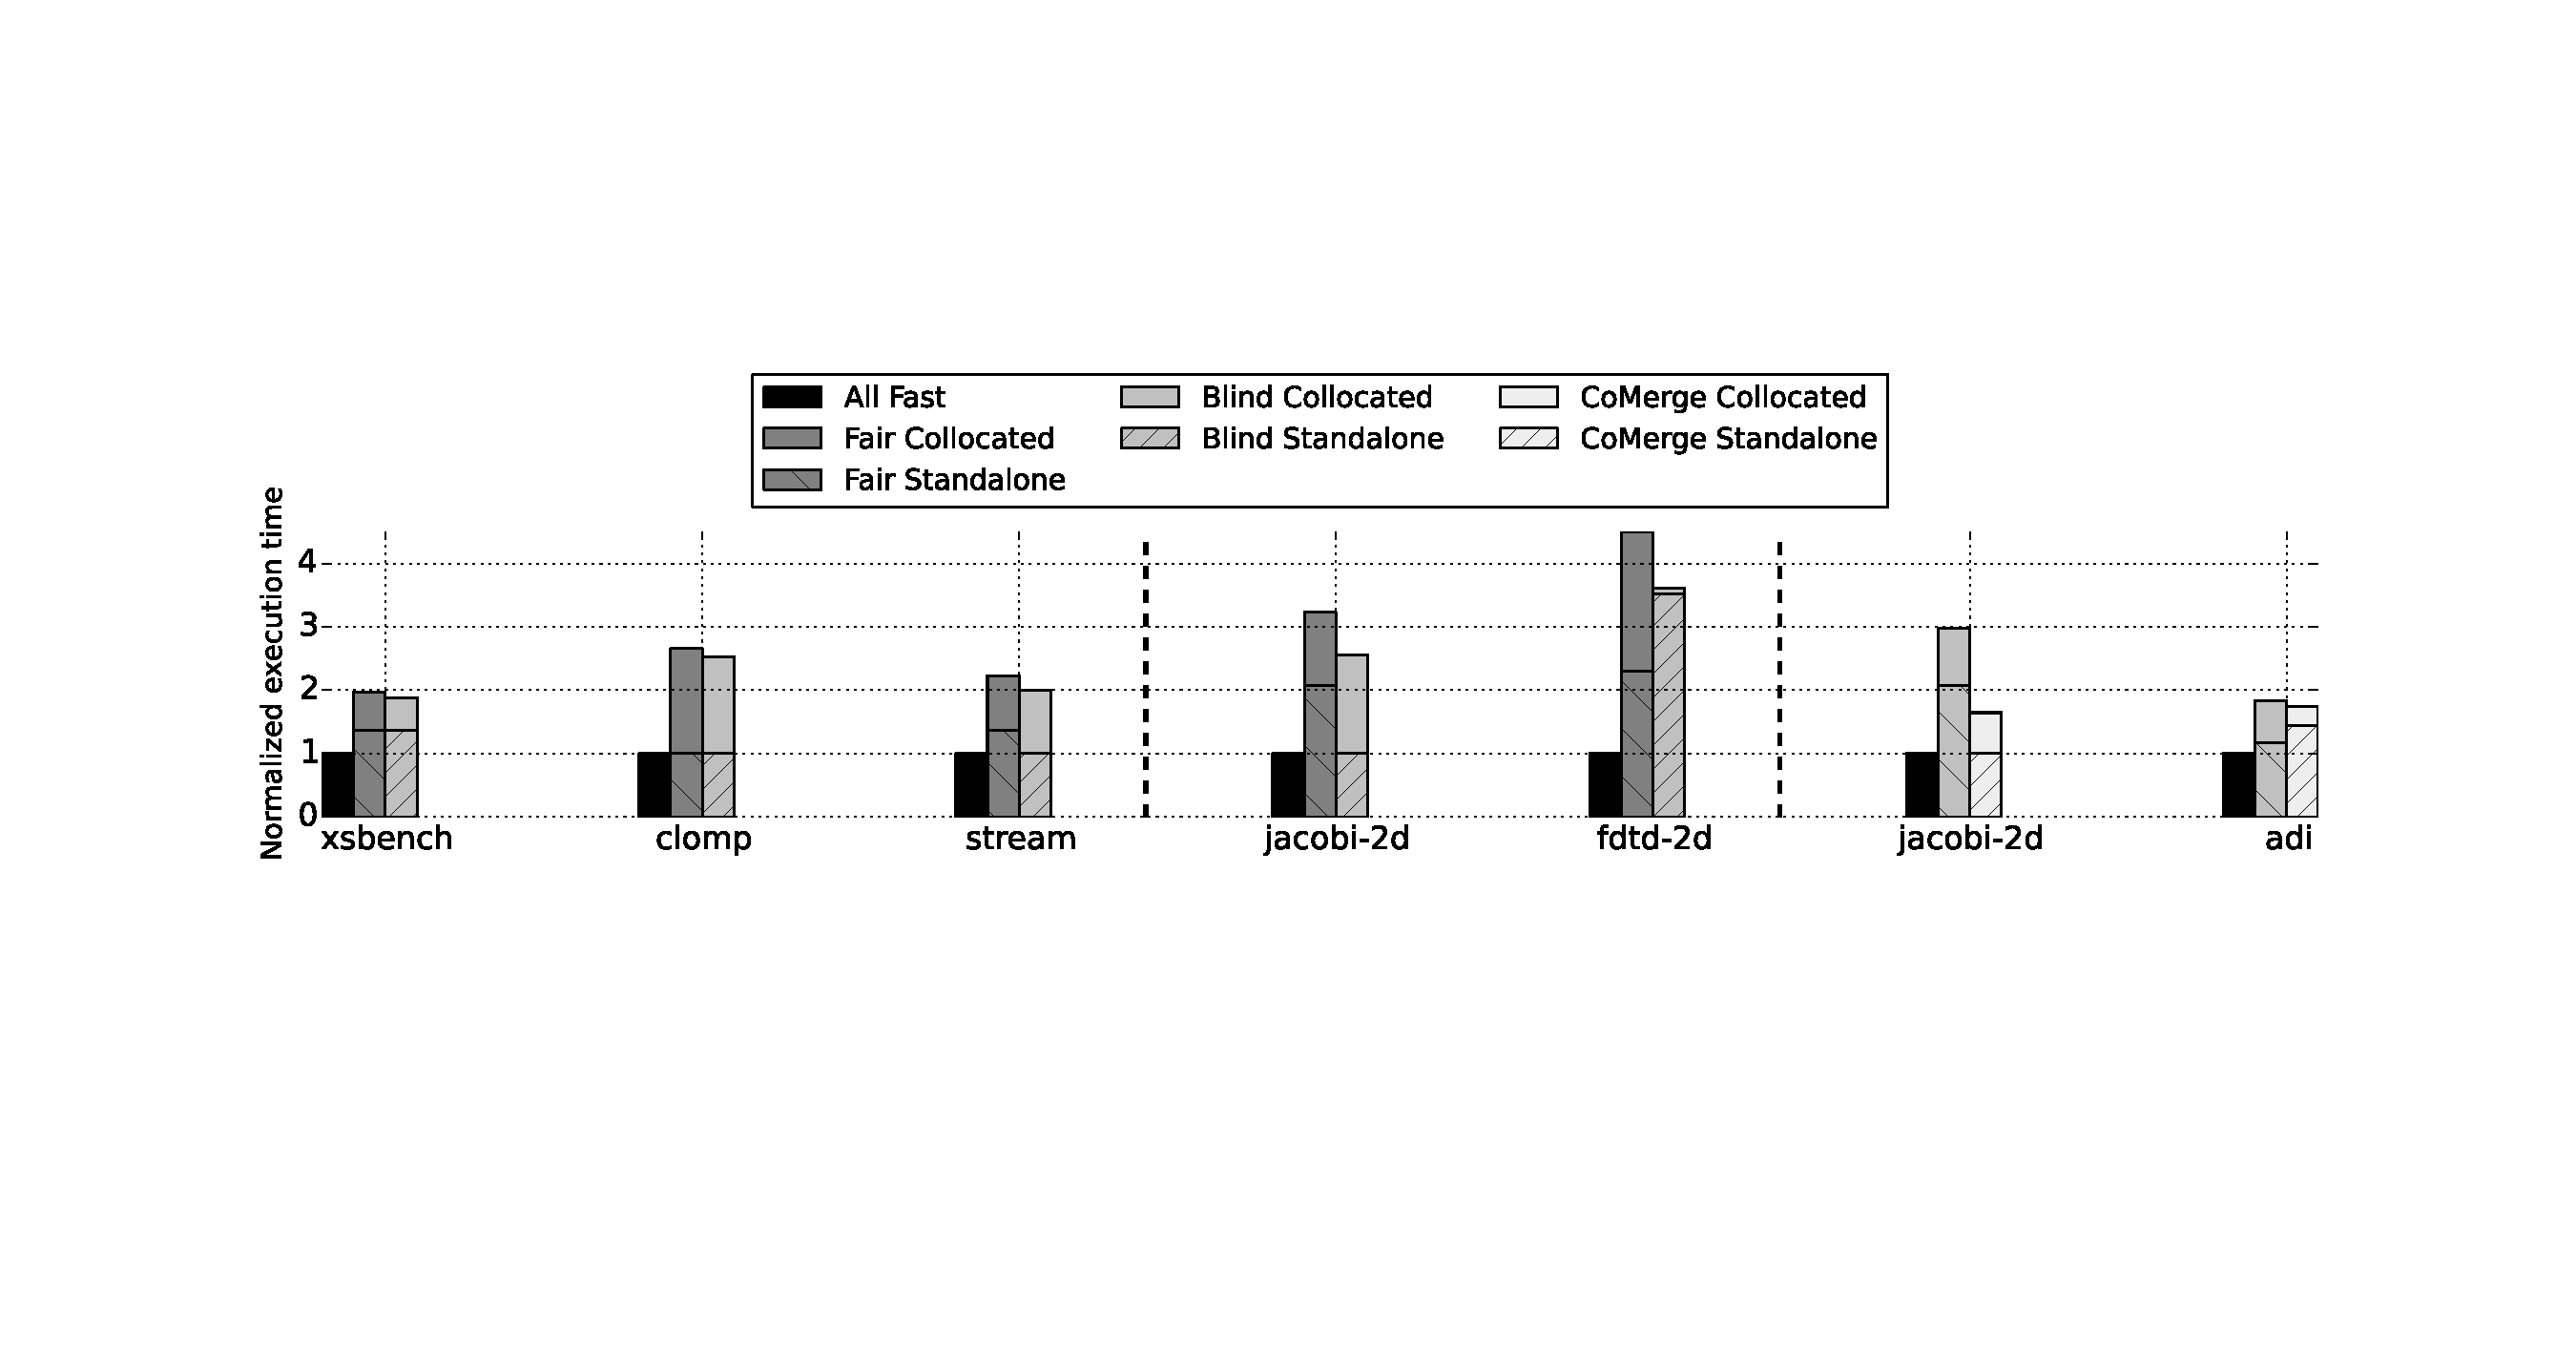
\includegraphics[width=\linewidth]{figures/tiering2.pdf}

      \captionsetup{labelformat=empty}

\caption{Execution time slowdown from `all-in-DRAM' for three different collocation combinations (separated with dashed lines). The shaded parts refer to the slowdown caused by data tiering. The unshaded parts depict the additional slowdown due to collocation.}
%  \label{fig:static}  
  \end{subfigure}

\begin{subfigure}{\linewidth}
  \begin{subfigure}{0.425\linewidth}
  	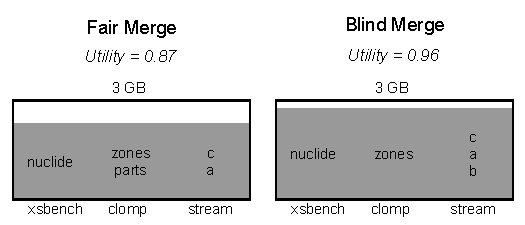
\includegraphics[width=\linewidth]{figures/tiering2a.pdf}
      \captionsetup{labelformat=empty}
  	\caption{Collocation of XSBench, CLOMP, STREAM}
  \end{subfigure}%  
     \begin{subfigure}{0.3\linewidth}
  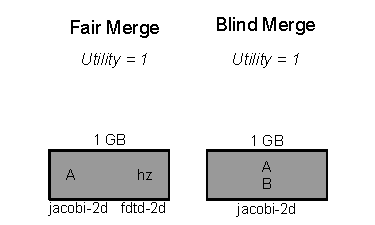
\includegraphics[width=\linewidth]{figures/tiering2b.pdf}
      \captionsetup{labelformat=empty}
    \caption{Collocation of jacobi-2d, fdtd-2d}
    \end{subfigure}%  
     \begin{subfigure}{0.3\linewidth}
     \centering
  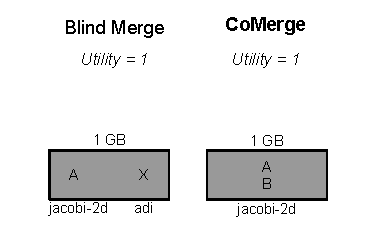
\includegraphics[width=\linewidth]{figures/tiering2c.pdf}
      \captionsetup{labelformat=empty}
    \caption{Collocation of jacobi-2d, adi}
    \end{subfigure}  
          \captionsetup{labelformat=empty}
  \caption{Utility and objects allocated in FastMem. }
  \end{subfigure}
  \caption{Comparison of Fair Merge, Blind Merge and CoMerge schemas for three different collocation combinations.}
    \label{fig:tiering2}

    \vspace{-0.1in}



\end{figure*}

Static partitioning techniques are essentially just applying the data tiering solutions to environments with even more restricted capacity. Especially in cases with very limited FastMem capacity, each placement decision can be crucial. 
In this section, we leverage the fact that the benefit factor values provide a normalized metric that captures the impact of the different application data structures on the overall workload sensitivity to execution over slower memory. We explore memory sharing schemas, so as to maximize the overall FastMem utility and facilitate decisions that increase performance across all applications, even if that restricts the fair usage of the shared FastMem.	
The following sharing policies merge the data structures of all collocated applications into a global object pool, where each object can be identified by the application where it belongs, its size and its benefit factor value. Then, they place objects into FastMem in descending order of benefit factor value, until total FastMem capacity is full. This is essentially a greedy algorithm, 
that can have two variances. \\

\noindent{\bf Fair merge.} This technique orders the objects of all collocated applications by merging them in descending benefit factor order and choosing from a different workload each time.
This schema ensures fairness, because it guarantees that all applications will be able to allocate part of their dataset in FastMem, if there is enough available capacity. It is susceptible to unfair cases, though, where 
an application with one object of significant size and high benefit factor, may take up the majority of the available FastMem space. Also, the application order of choice impacts the data tiering, as there may be cases where some applications may have more objects in FastMem than others. We define this order with respect to the overall dataset size, so as to prioritize applications with bigger memory footprint. \\
\noindent{\bf Blind merge.} This is a direct mergesort of the actual benefit factor values of the different data objects across the co-existing kernels, ignoring any application order. It allows for possible scenarios where one application may get full priority over another one, 
because its objects have bigger benefit factor values than the objects of the other kernels.\\

\begin{comment}
\begin{table}[t]
\centering
  \begin{tabular}{|p{1.2cm}||p{3cm}||p{3cm}|} \hline
    Kernel & Fair merge & Blind merge \\\hline \hline
    jacobi-2d 	& A (F) > B (S) &  A (F) > B (F) \\\hline
    fdtd-2d 	& hz (F) > ey (S) > ex (S) & hz (S) > ey (S) > ex (S) \\\hline
        xsbench 	& nuclide (F) > energy (S) & nuclide (F) > energy (S) \\\hline
    clomp	 	& zones (F) > parts (F) & zones (F) > parts (S) \\\hline
    stream 		& c (F) > a (F) > b (S) & c (F) > a (F) > b (F) \\\hline
  \end{tabular}
  \caption{Data tiering due to the capacity restrictions over fair and blind merge schemas. (F) indicates object allocation in FastMem, (S) in SlowMem.}
  \label{tbl:tiering_merge}
    %\vspace{-0.3in}
\end{table}
\end{comment}

%\begin{figure}[t]
  %\centering
%  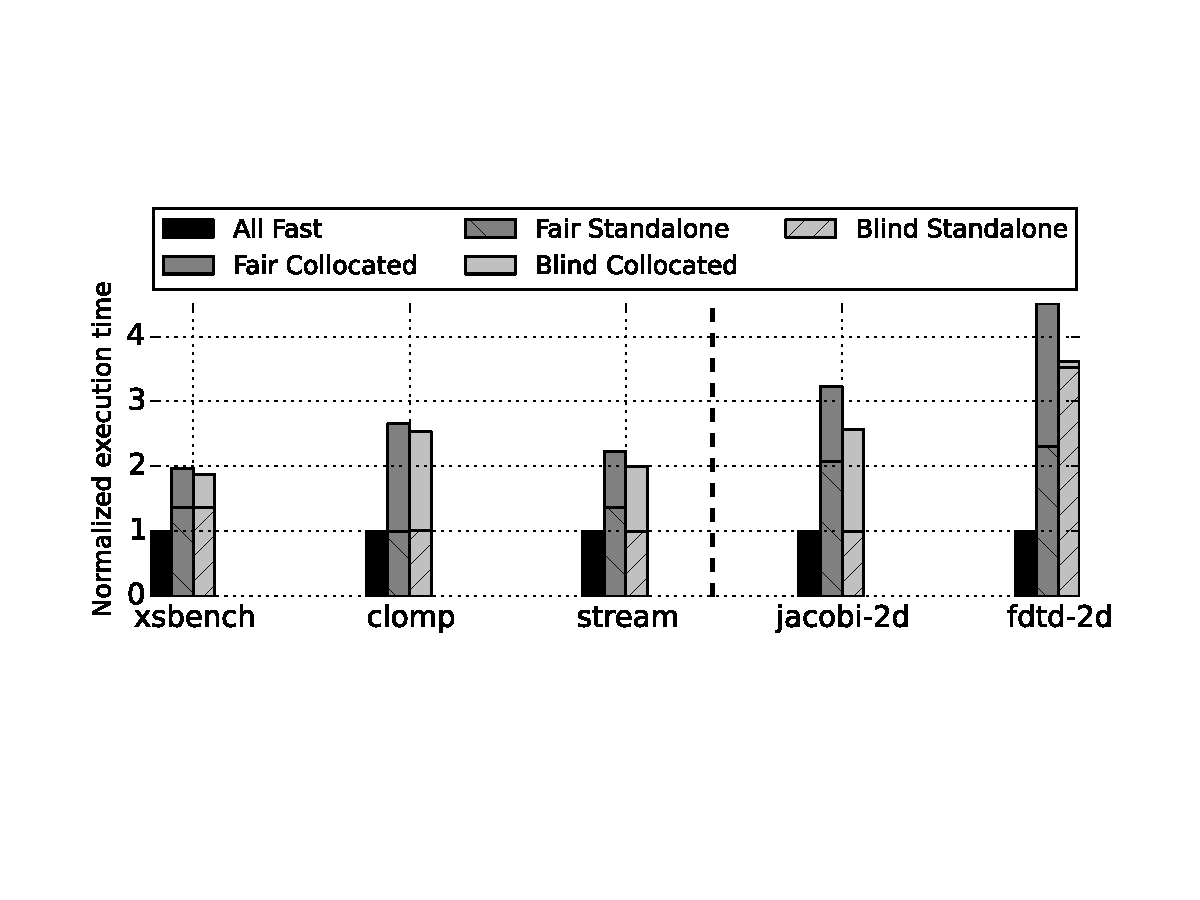
\includegraphics[width=\columnwidth]{figures/merge.pdf}
  %\caption{Execution time slowdown from 'all-in-FastMem' for the fair and blind merge schemas and two different collocation scenarios. The shaded parts refer to the slowdown caused by data tiering. The unshaded parts depict the additional slowdown due to collocation.}
  %\label{fig:merge}
%    \vspace{-0.3in}
%\end{figure}

%\subsubsection
\vspace{1ex}
\noindent{\bf\em CORAL Experiments}
\vspace{0.3ex} 

\noindent First, we experiment using the CORAL benchmarks configuration as in the previous subsection. The aggregate memory footprint is 4.1 GB and the available FastMem is 3 GB. The application data structures now form a global object pool whose sizes and benefit factor values are listed in table~\ref{tbl:tiering}. In the fair merge schema, we choose one object at a time from every application, in descending order of overall dataset size. Thus, we choose one object from STREAM, then CLOMP and then XSBench and repeat until FastMem cannot fit any other whole objects. The objects allocated in FastMem are depicted in Figure~\ref{fig:tiering2}. Similarly, for the blind merge schema we sort all objects from the global pool, in descending absolute benefit factor value and place them in FastMem until no other object fits. 
Figure~\ref{fig:tiering2} also shows the execution time slowdown of each collocated application due to data tiering and collocation.

To begin with, as far as the slowdown due to data tiering is concerned, we see that it is similar in both fair and blind merge schemas. This is due to the fact that XSBench has the same data tiering, whereas CLOMP has a trivial benefit factor object in SlowMem and STREAM has all of its dataset in FastMem in the blind merge schema. 
Second, regarding the slowdown due to collocation we see that all applications benefit from the blind merge schema. This schema enables the optimal global data placement, because it keeps in FastMem the objects from XSBench and CLOMP that have a really high benefit factor and allocates all the dataset of STREAM in FastMem. This global data tiering, allows applications to benefit both from low access times to the objects that are critical to performance and allocated in FastMem. Additionally, it maintains the low impact to performance of the objects with low benefit factor, due to the efficient utilization of the SlowMem bandwidth. This was not the case in the static partitioning schemas, where objects with low benefit factor that were allocated in SlowMem would impact significantly the collocation slowdown, due to their accesses being interleaved with objects of high benefit factor allocated in SlowMem, inflicted by the un-intelligent data tiering imposed by the partitioning schema. Finally, we observe that the blind merge schema allows almost optimal FastMem utility of 0.96, compared to 0.87 with the fair merge schema. 

Overall, the blind merge schema facilitates an optimal global data placement across co-running applications and high FastMem utility, leveraging the low access time for objects in FastMem with high benefit factor, as well as maintaining the low impact to performance slowdown of objects with low benefit factor, due to the efficient usage of the SlowMem bandwidth.\\

\vspace{1.5ex}
\noindent{\bf\em Polybench Experiments}
\vspace{0.3ex} 

\noindent We now experiment with a setup where the overall FastMem capacity is 1 GB, so as to highlight the importance of each individual choice in an environment with restricted FastMem capacity. We collocate 
two high sensitivity kernels jacobi-2d and fdtd-2d, which have data objects of 500 MB each. Figure~\ref{fig:tiering2} shows the tiering when applying fair and blind merge. 
More specifically, fair merge will choose the object with highest benefit factor from each application. In contrast, blind merge prioritizes jacobi-2d over fdtd-2d, because its data objects have 
higher overall benefit factor values, as you can refer back to table ~\ref{tbl:tiering}. Figure ~\ref{fig:tiering2} shows the execution time of each collocated kernel, normalized to the baseline case where all data could fit into FastMem in 
standalone execution. 
We can first observe the impact of data tiering, especially in the case of fdtd-2d, where blind merge is equivalent to the worst case scenario, where all objects are allocated in SlowMem. 
However, we notice that blind merge leads to less overall slowdown during collocation. This can be potentially attributed to the fact that memory requests can be serviced in parallel from FastMem and SlowMem for the different applications due to the better bandwidth usage distribution, even 
though accessing SlowMem maybe incur higher latency. Overall, prioritizing one application over another one, even though it's not fair, it may lead to better performance across both applications. 


\begin{comment}
\begin{table}[t]
\centering
  \begin{tabular}{|p{1.2cm}||p{3cm}||p{3cm}|} \hline
    Kernel & Blind merge & Blind co-merge \\\hline \hline
    jacobi-2d 	& A (F) > B (S) &  A (F) > B (F) \\\hline
    adi 	& X (F) > B (S) > A (S) & X (S) > B (S) > A (S) \\\hline
  \end{tabular}
  \caption{Data tiering due to the capacity restrictions over blind merge and co-merge schemas. (F) indicates object allocation in FastMem, (S) in SlowMem.}
  \label{tbl:co-merge}
     %\vspace{-0.3in}
\end{table}
\end{comment}

%\begin{figure}[t]
  %\centering
  %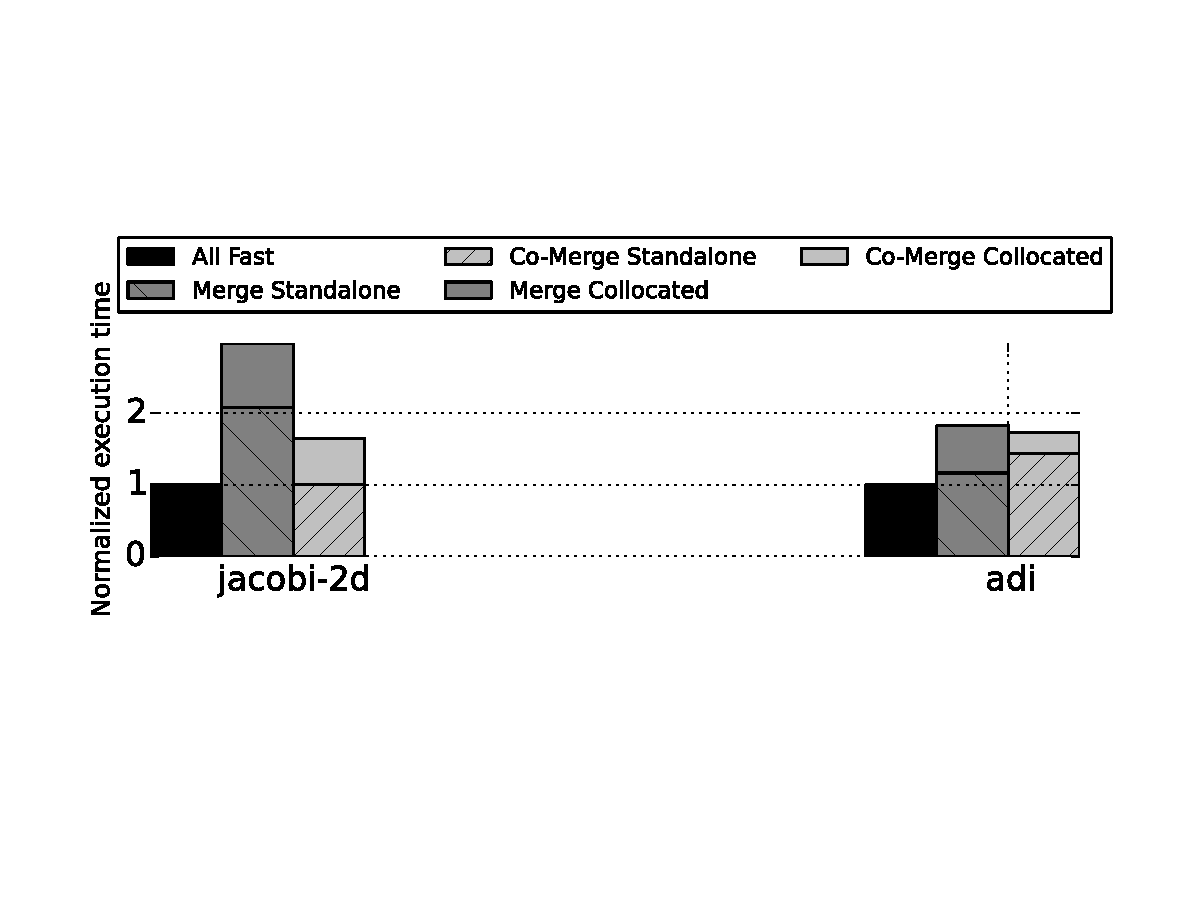
\includegraphics[width=\columnwidth]{figures/comerge.pdf}
%  \caption{Execution time slowdown from 'all-in-FastMem' for the blind merge and co-merge schemas. 
  %The shaded parts refer to the slowdown caused by data tiering. The unshaded parts depict the additional slowdown due to collocation.}
  %\label{fig:co-merge}
    %  \vspace{-0.3in}
%\end{figure}

We now apply the blind merge schema, when collocating high and low sensitivity kernels, jacobi-2d and adi.  We observe in Figure~\ref{fig:tiering2} that for the blind merge schema, the impact of collocation compared to standalone and baseline, is much more significant for jacobi-2d as it is a high sensitivity kernel, 
rather than adi that has very low sensitivity. Therefore, we see that jacobi-2d is in greater need of FastMem, so as to mitigate the performace slowdown. 
However, the absolute benefit factor values do not capture the overall sensitivity of the application. This is the reason why, we propose a {\it co-benefit factor}, which scales the current benefit factor by a value that 
corresponds to the overall slowdown of the application execution time when all data is allocated in SlowMem compared to FastMem, which is the value that essentially captures the overall application sensitivity level. 
\[Co-Benefit(O) = floor(\frac{S}{F})*\frac{t(O)-S}{F-S}\]
Table~\ref{tbl:tiering} includes the co-benefit values for the different objects of every application. We note that non-sensitive kernels have zero co-benefit values, because they should not get prioritized for placement in FastMem, 
as allocation in SlowMem does not impact overall performace. \\

\noindent{\bf CoMerge.} This is a direct mergesort of the {\it co-benefit factor} values of the data structures across all collocated applications. Objects are placed in FastMem in descending co-benefit factor order, until no other object can be placed due to capacity restrictions. 
Since the co-benefit factor now captures the overall application sensitivity to SlowMem, objects from more sensitive workloads get higher weight thus priority in the above sorting.
 If the collocated applications belong in the same sensitivity level, then the technique is the same with the blind merge, due to the way the co-benefit factor is calculated to scale with the level of sensitivity. 
 
Therefore, back in the example of Figure~\ref{fig:tiering2} we see that a CoMerge policy will prioritize jacobi-2d over adi and this data arrangement mitigates the 
slowdown for both kernels, even more significantly for jacobi-2d that is a high sensitivity kernel. \\

\vspace{0.8ex}
\noindent{\bf\em Takeaways}
\vspace{0.3ex} 

\noindent In conclusion, we propose CoMerge, a memory sharing technique that can provide the most intelligent global data tiering of application data structures that are collocated in shared heterogeneous memory environments. First, CoMerge is able to maximize the FastMem utility due to the fact that is a memory sharing technique. Second, it can efficiently mitigate the performance slowdown across all collocated applications, via the use of co-benefit factor values that are able to capture the exact impact of a data structure to the application performance in shared environments, incorporating the overall application sensitivity to SlowMem. CoMerge sorts the global object pool in descending co-benefit factor value and allocates them in FastMem until capacity is full. This technique leverages both the fast access time to FastMem for objects with high benefit factor, as well as the  SlowMem bandwidth for objects with low benefit factor. 
